\documentclass[]{scrartcl}
\usepackage{graphicx}
\usepackage{geometry}
\geometry{
	a4paper,
	total={170mm,257mm},
	left=20mm,
	top=20mm,
}


%opening
\title{Software Design Description}
\author{Brandon Smith, Nieka Gutenberger, Joseph Coppin, Ryan Frazier, Trevor Jewkes}

\begin{document}

\maketitle
\pagebreak
\section{Software Design}
\subsection{Login Screen}

\centerline{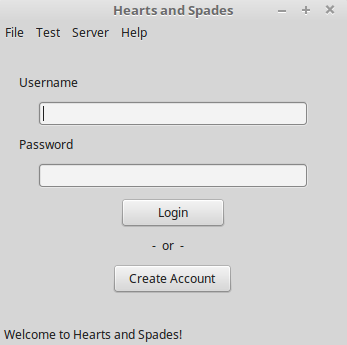
\includegraphics{LoginScreen.png}}

This screen is the first screen the user will see.  It has a text box for the user to enter a user name and password.  It also has two buttons a “login” which sends the username and password to the server, and brings up the lobby screen; and a “Create Account” button which takes the user to screen where they can create their account prior to playing games. 

The account creation has text fields for all the information needed to create an account including Name, “Username”, “Password”  and “Verify Password”,  Finally the page includes a “Create Account” button which sends all information to the server so it can create the account.  

\subsection{Main Menu}
\centerline{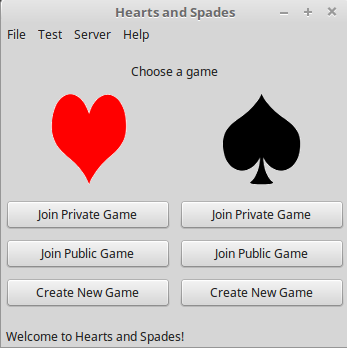
\includegraphics{SelectGame.png}}

This screen is the main menu for the Game, it is divided in half with one half related to the game of Hearts, and the other half for the game of Spades.  Each half includes three buttons, “Join Private”, “Join Public” and “Create New”.  The “Join Private” brings up a screen which allows the user enter the name of the game they want to join.  The “Join Public” will tell the server to assign the user to the first available  public game, if no game is available the server will create a new game with the user and three AI players.  Finally the “Create New” button will bring up a screen which asks for the users preferences to create a new game.

\centerline{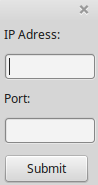
\includegraphics{ServerSelection.png}}

When connecting to the server, a menu option is available to specify the IP Address and Port number for the server.


\subsection{Game Play}
\centerline{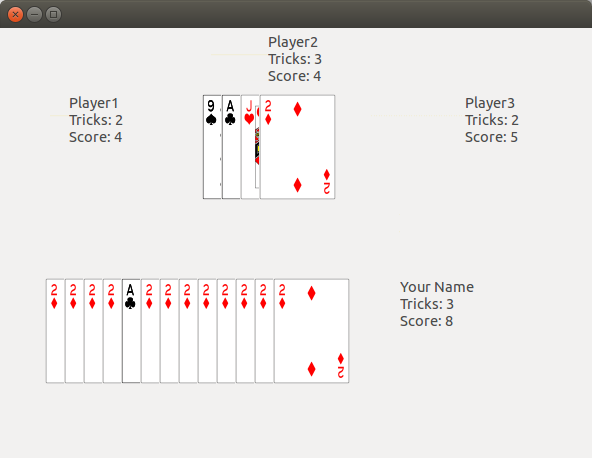
\includegraphics{game_board.png}}
This screen will be the view that will be use for play of the game. Since Spades and Hearts have the same basic set-up we can use the same view for both. It shows the players hand along with the scores of the other players. Placing bids and passing cards fit within the gameplay screen.


\subsection{End-of-Game}
\centerline{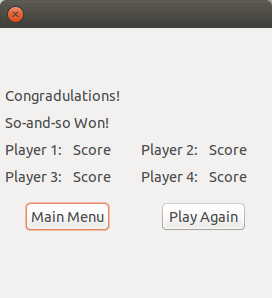
\includegraphics{end_game.png}}
This the End-of-Game screen. It will display the winner of the game along with the final scores for the game.

 There are two buttons, "Play Again" and "Main Menu". The "Play Again" button is used to play again with the same players. The "Main Menu" button will return the user to the main menu.
\end{document}
